\chapter{Simultated Comparison of Neuromuscular and Impedance Controllers}\label{sec:control_sim}

\graphicspath{{chapters/control_simulation/figures/}}

\emph{Material in this section based partially on
\citet{thatte2016toward}\cite{thatte2016toward} and
\citet{thatte2014towards}\cite[0.25in]{thatte2014towards}} \linebreak

To evaluate the potential of neuromuscular prosthesis control to improve amputee
gait robustness, we construct a simulation of an amputee walking on a powered
prosthesis and perform optimizations to identify parameters that lead to robust
locomotion over rough terrain. We then compare the performance of the proposed
control to that of impedance control and find that the proposed control improves
robustness to elevation changes and unexpected deviations from nominal walking,
suggesting that it may help amputees prevent trips and falls
(\cref{fig:distsWalked}).

\section{Planning Approach Methods}
The trip avoidance control we propose involves (1) estimating the position and
orientation of the leg (\cref{sec:hip_kalman}), (2) predicting the future hip
angles and heights (\cref{sec:predict_gp}), and (3) planning corresponding knee
and ankle trajectories such that the heel and toe will not contact the ground
prematurely (\cref{sec:traj_plan}).

\subsection{Extended Kalman Filter for estimating Leg Position/Orientation}
\label{sec:hip_kalman}

To estimate the position and orientation of the leg, we employ an EKF that fuses
information from a LIDAR distance sensor (SICK OD1000), an IMU (YEI Technologies
3-Space sensor), and encoders on the prosthesis (Renishaw Resolute, Netzer
DS-25). The EKF filters the nonlinear, discrete-time dynamics given by
\begin{align}
    x_{t} = \begin{bmatrix} q_t \\ p_t \\ \dot{p}_t \end{bmatrix}
        &= \begin{bmatrix} f_\tn{gyro}(\omega_t) & 0 & 0 \\
            0 & I_{3\times3} & \Delta t  I_{3\times3}\\
            0 & 0 & I_{3\times3} \end{bmatrix} x_{t-1} \notag \\
        &\quad+ \begin{bmatrix} 0 \\ \frac{1}{2} \Delta t^2 I_{3\times3} \\ 
            \Delta t I_{3\times3} \end{bmatrix} 
        \begin{bmatrix} R_\tn{OI}(q_{t-1}) a_t - \begin{bmatrix} 0 \\ 0 \\ g 
            \end{bmatrix} \end{bmatrix} + w_t \label{eq:dynamics}\\
            &= f(x_{t-1}, u_t) + w_t  \notag ,
\end{align}
where $q$ is the quaternion orientation, $R_\tn{OI}$ and $p$ are the rotation
matrix and position of the IMU in inertial coordinates, $\omega$ is the angular
rate measured by the gyroscope, $f_\tn{gyro}$ integrates the gyroscope rate to
update the orientation, $a$ is the accelerometer measurement, $u_t =
\left[\omega_t, a_t \right]^T$, and $\Delta t$ is the integration time step
(\unit[1]{ms}). 

The dynamics are corrupted by process noise $w_t \sim \mathcal{N}(0, Q_t)$ due
to the inaccuracy of the IMU's measurement of the true acceleration and angular
velocity. Consequently, $Q_t$ is given by
\begin{align}
    Q_t = \left. \frac{\partial f}{\partial u} \right|_{x_{t-1}, u_t}
        \begin{bmatrix} \sigma_\omega^2 I_{3\times3} & 0 \\ 
            0 & \sigma_a^2 I_{3\times3} \end{bmatrix}
        \left. \frac{\partial f}{\partial u} \right|_{x_{t-1}, u_t}^T,
\end{align}
where $\sigma_\omega^2$ and $\sigma_a^2$ are the gyroscope and accelerometer
measurement variances, respectively.

\begin{marginfigure}
    \centering
    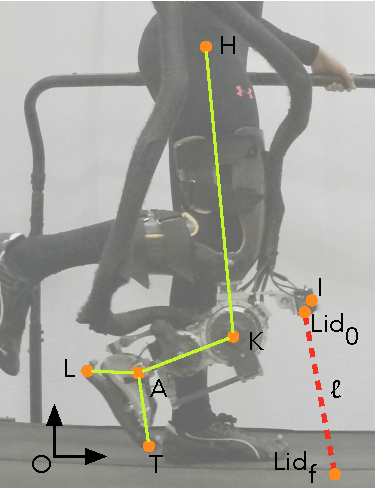
\includegraphics[width=\columnwidth]{kinematics}
    \caption{Kinematic model of the user and prosthesis used for state
    estimation and motion planning. The model includes the hip (H), knee (K),
    ankle (A), heel (L) and toe points (T). Additionally, the start ($Lid_0$)
    and end ($Lid_f$) points of the LIDAR beam (with length $\ell$) are
    indicated. The IMU is located at point $I$. Both the LIDAR and IMU are
    mounted to the thigh portion of the powered knee-and-ankle
    prosthesis.}\label{fig:kinematics}
\end{marginfigure}

To estimate the pose given our sensor measurements, we follow a standard EKF
procedure \citep{anderson1979optimal}, reviewed here for completeness. The EKF
state estimation process has two steps: First, we \emph{predict} the next state
distribution by forward-propagating the mean $\hat{x}_{t-1|t-1}$ and covariance
of the state estimate $\Sigma_{t-1|t-1}$ using the dynamics given by
\cref{eq:dynamics},
\begin{align}
    \hat{x}_{t|t-1} &= f(\hat{x}_{t-1|t-1}, u_t) \\
    \Sigma_{t|t-1} &= F_t \Sigma_{t-1|t-1} F_t^T + Q_t,
\end{align}
where $F_t = \left. \partial f / \partial x \right|_{\hat{x}_{t-1|t-1}}$.

Next, we incorporate information from noisy sensor observations to \emph{update}
the state estimate. To do this, we utilize a observation model given by $z_t =
h(x_t) + v_t$, where $v_t \sim \mathcal{N}\left(0, R \right)$, and the following
update equations:
\begin{align}
    K_t &= \Sigma_{t|t-1} H_t^T 
        {\left(H_t \Sigma_{t|t-1} H_t^T + R\right)}^{-1} \\
    \hat{x}_{t|t} &= \hat{x}_{t|t-1} + K_t \left(z_t - h(\hat{x}_{t|t-1}) \right) \\
    \Sigma_{t|t} &= \left(I - K_t H_t \right) \Sigma_{t|t-1}
\end{align}
where $z_t$ are the actual sensor measurements and $H_t = \left. \partial h /
\partial x \right|_{\hat{x}_{t-1|t}}$.

The observations in our EKF formulation use the kinematic model shown in
\cref{fig:kinematics}. We calibrate this model using ground truth data from a
VICON motion capture system. In our application we incorporate three
observations:
\begin{enumerate}
\item The expected acceleration vector points up in the global coordinate frame,
\begin{align} 
    h_1(x_t) &= {\left\{R_\tn{OI}(q) \right\}}_\textrm{row 3} \\
    z_1 &= a
\end{align}

\item The expected LIDAR measurement given the position of the IMU,
\begin{align}
    h_2(x_t) &= \left\{\ell : \left\{ p_\tn{OLID_f}\left(x_t, \ell \right)
        \right\}_\tn{row 3} = 0\right\} \\
    z_2 &= \ell_\tn{meas},
\end{align}
where $p_\tn{OLID_f}$, is the location of the laser beam endpoint represented in
the global coordinate system, $\ell = \lVert
\overrightarrow{\tn{LID_0}\tn{LID_f}} \rVert$ is the modeled laser beam length,
and $\ell_\tn{meas}$ is the actual measured LIDAR distance.

\item During stance, the toe point coincides with the origin (active
\unitfrac[200]{m}{s} after stance begins until toe-off)
\begin{align}
    h_3(x_t) &= p_\tn{OT}(x_t, \theta_\tn{k}, \theta_\tn{a}) \\
    z_3 &= {[0 \ 0 \ 0]}^T
\end{align}
where $p_\tn{OT}$ is the location of the toe in the inertial frame, and
$\theta_\tn{k}$ and $\theta_\tn{a}$ are the measured knee and ankle angles.
\end{enumerate}

The measurement noise for these observations is given by
\begin{align}
    R = \begin{bmatrix} \sigma_a^2 I_{3\times3} & 0 \\
        0 & \sigma_l^2 \end{bmatrix}
\end{align}
during swing and
\begin{align}
    R = \begin{bmatrix} \sigma_a^2 I_{3\times3} & 0 & 0 \\
        0 & \sigma_\ell^2 & 0 \\
        0 & 0 & \sigma_f^2 I_{3\times3} \end{bmatrix}
\end{align}
during stance. In these equations, $\sigma_a^2$ is the accelerometer variance,
$\sigma_\ell^2$ is the LIDAR measurement variance, and $\sigma_f^2$ is the foot
position variance.

To further improve the EKF's state estimate, we enforce a number of
constraints using the methods provided by \citet{gupta2007kalman}. Specifically,
we enforce three equality constraints:
\begin{enumerate}
\item First, we require that the quaternion has unit norm
\begin{align}
    1 = q_1^2 + q_2^2 + q_3^2 + q_4^2.
\end{align}

\item Second, we prevent the yaw component of the orientation $q$ from drifting.
To do this, we convert the $q$ to ZYX Euler angles and enforce $\phi_z = 0$, 
\begin{align}
    0 = \func{atan2}{2 (q_1 q_4 + q_2 q_3), 1 - 2 (q_3^2 + q_4^2)}.
\end{align}

\item Finally, during stance we further constrain the toe's $x$ and
$y$-coordinates to 0,
\begin{align}
    \begin{bmatrix} 0 \\ 0 \end{bmatrix} 
        &= {\left\{p_\tn{OT}(x_t, \theta_\tn{k}, \theta_\tn{a}) 
            \right\}}_\textrm{rows 1 and 2}.
\end{align}
\end{enumerate}

\noindent In addition, we use inequality constraints to ensure the toe and heel
do not penetrate the ground,
\begin{align}
    0 &\le {\left\{p_\tn{OT}(x_t, \theta_\tn{k}, \theta_\tn{a}) 
        \right\}}_\textrm{row 3} ,\\
    0 &\le {\left\{p_\tn{OL}(x_t, \theta_k, \theta_a) 
        \right\}}_\textrm{row 3}.
\end{align}

\noindent We enforce these constraints by solving the following quadratic
program after each update step,
\begin{align}
\hat{x}_{t|t}^\tn{proj} 
    &= {\argmin_x \left(x - \hat{x}_{t|t} \right)}^T \Sigma_{t|t}^{-1} 
        \left(x - \hat{x}_{t|t} \right),
\end{align}
such that
\begin{align}
    A_\tn{eq} x &= b_\tn{eq}, \\
    A_\tn{ineq} x &= b_\tn{ineq},
\end{align}
where $A_\tn{eq}$,  $b_\tn{eq}$, $A_\tn{ineq}$, and $b_\tn{ineq}$ are derived
from linearizing the equality and inequality constraints.

\begin{marginfigure}[-1in]
    \centering
    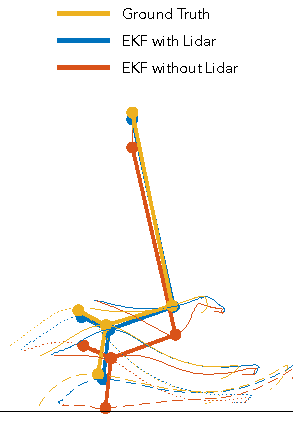
\includegraphics[width=\columnwidth]{ekf_fig}
    \caption{Trajectories of extended Kalman Filter (EKF) estimate of the
    position of the leg during swing (blue). Ground truth positions given by
    motion capture (yellow). EKF estimate without LIDAR information shown in
    red. Thick lines show the leg configuration at peak toe height during swing.
    Dotted lines indicate heel trajectories while dashed lines show the toe
    trajectories. Knee and ankle trajectories given by solid lines.}\label{fig:ekf}
\end{marginfigure}

To identify the appropriate parameters of the Kalman filter, we collected ground
truth training and testing kinematic data using a Vicon motion capture system
and optimized the parameters of the EKF to minimize the error of the kinematic
estimate. The parameters we optimized were the rotation of the LIDAR with
respect to the hip, the translation between the LIDAR and the IMU, and
$\sigma_\omega$, $\sigma_a$, $\sigma_\ell$, and $\sigma_f$. 

\Cref{fig:ekf} shows an example of the resulting EKF estimates of the hip, knee,
ankle, heel, and toe positions during swing (blue stick figure and traces)
compared to the ground truth obtained from the motion capture system (yellow)
and an EKF estimate without the LIDAR sensor information integrated (red). Over
the entire test data set, the root mean squared error of the estimated heel and
toe positions during swing is \unit[18.6]{mm} for the EKF with LIDAR
information. In contrast, the EKF without LIDAR information has an error of
\unit[46.7]{mm}. Thus, including the LIDAR sensor data reduces the error by
60\%.

\begin{figure}[t]
    \centering
    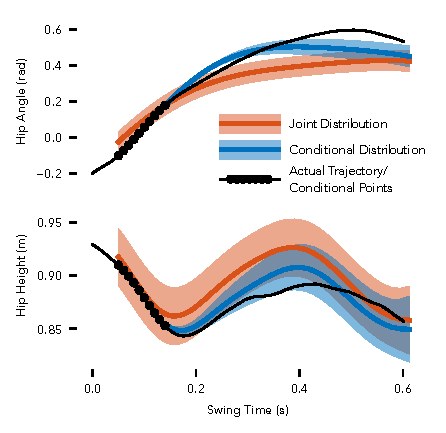
\includegraphics[width=\columnwidth]{gp_plots_w_legend}
    \caption{Example of hip angle and height trajectory predictions
    \unit[0.15]{s} into swing. The prediction algorithm uses the previous 10
    measured hip angles and heights (sampled at \unit[100]{Hz}, black dots)
    along with the learned joint distributions of hip angles/heights versus time
    (red) to obtain the conditional distributions of future hip angles/heights
    (blue). The planning algorithm uses the means of the conditional
    distributions to generate knee and ankle trajectories. The actual hip height
    and angle trajectories are shown in black.}
    \label{fig:gp_plots}
\end{figure}
\subsection{Gaussian Process Hip Trajectory Prediction}

\label{sec:predict_gp}
To predict the future hip angle and height trajectories, we train sparse
Gaussian process models using the FITC approximation \citep{snelson2007local}.
The sparse approximation ensures the computational complexity at test time is
independent of the training data set size, providing consistent real time
performance. Throughout the swing phase, the learned hip angle and height
distributions are conditioned on the swing trajectories completed so far to
predict the distribution of the future trajectories for the rest of the swing
(example shown in \cref{fig:gp_plots}). Our algorithm then uses the means of
these conditional distributions in the motion planning phase
(compare \cref{sec:traj_plan}). 

For example, to calculate the conditional mean of future hip angles, we first
compute the joint distribution of completed $(\theta_h^\tn{c})$ and future
$(\theta_h^\tn{f})$ hip angles,
\begin{align}
    \func{P}{\theta_h^\tn{c}, \theta_h^\tn{f}} &=
        \mathcal{N}\left(\mu_\tn{fitc}, \Sigma_\tn{fitc} 
            + K\left( t_\tn{joint}, t_\tn{joint} \right) \right) \\
    &= \mathcal{N}\left( 
        \begin{bmatrix} 
            \mu_\tn{c} \\ \mu_\tn{f} 
        \end{bmatrix},
        \begin{bmatrix} 
            \Sigma_{\tn{c},\tn{c}} & \Sigma_{\tn{c},\tn{f}} \\ 
            \Sigma_{\tn{f},\tn{c}} & \Sigma_{\tn{f},\tn{f}} 
        \end{bmatrix}
        \right),
\end{align}
where $\mu_\tn{fitc}$ and $\Sigma_\tn{fitc}$ are obtained from equation 11 in
\citep{snelson2007local} and $K\left( t_\tn{joint}, t_\tn{joint}\right)$ is an
additional noise term given by a rational quadratic kernel
\citep{rasmussen2004gaussian} that correlates the predicted angles across time,
which results in smooth predicted trajectories. The mean of the conditional
distribution $\func{P}{\theta_h^\tn{f}|\theta_h^\tn{c}}$ is then given by
\begin{align}
    \mu_\tn{f}^\tn{cond} = \mu_\tn{f} + \Sigma_{\tn{f},\tn{c}}
        \Sigma_{\tn{c},\tn{c}}^{-1}\left(\mu_\tn{c} - \theta_h^\tn{c} \right).
    \label{eq:gp_cond_mean}
\end{align}
As the inversion of $\Sigma_{\tn{c},\tn{c}}$ is the most computationally
expensive component of \cref{eq:gp_cond_mean}, we use at most the last 10 hip
angles and heights (sampled at \unit[100]{Hz}) when calculating the conditional
mean (compare \cref{fig:gp_plots}).

\subsection{Trajectory Planning Quadratic Program Formulation}
\label{sec:traj_plan}

\begin{pagefigure}
    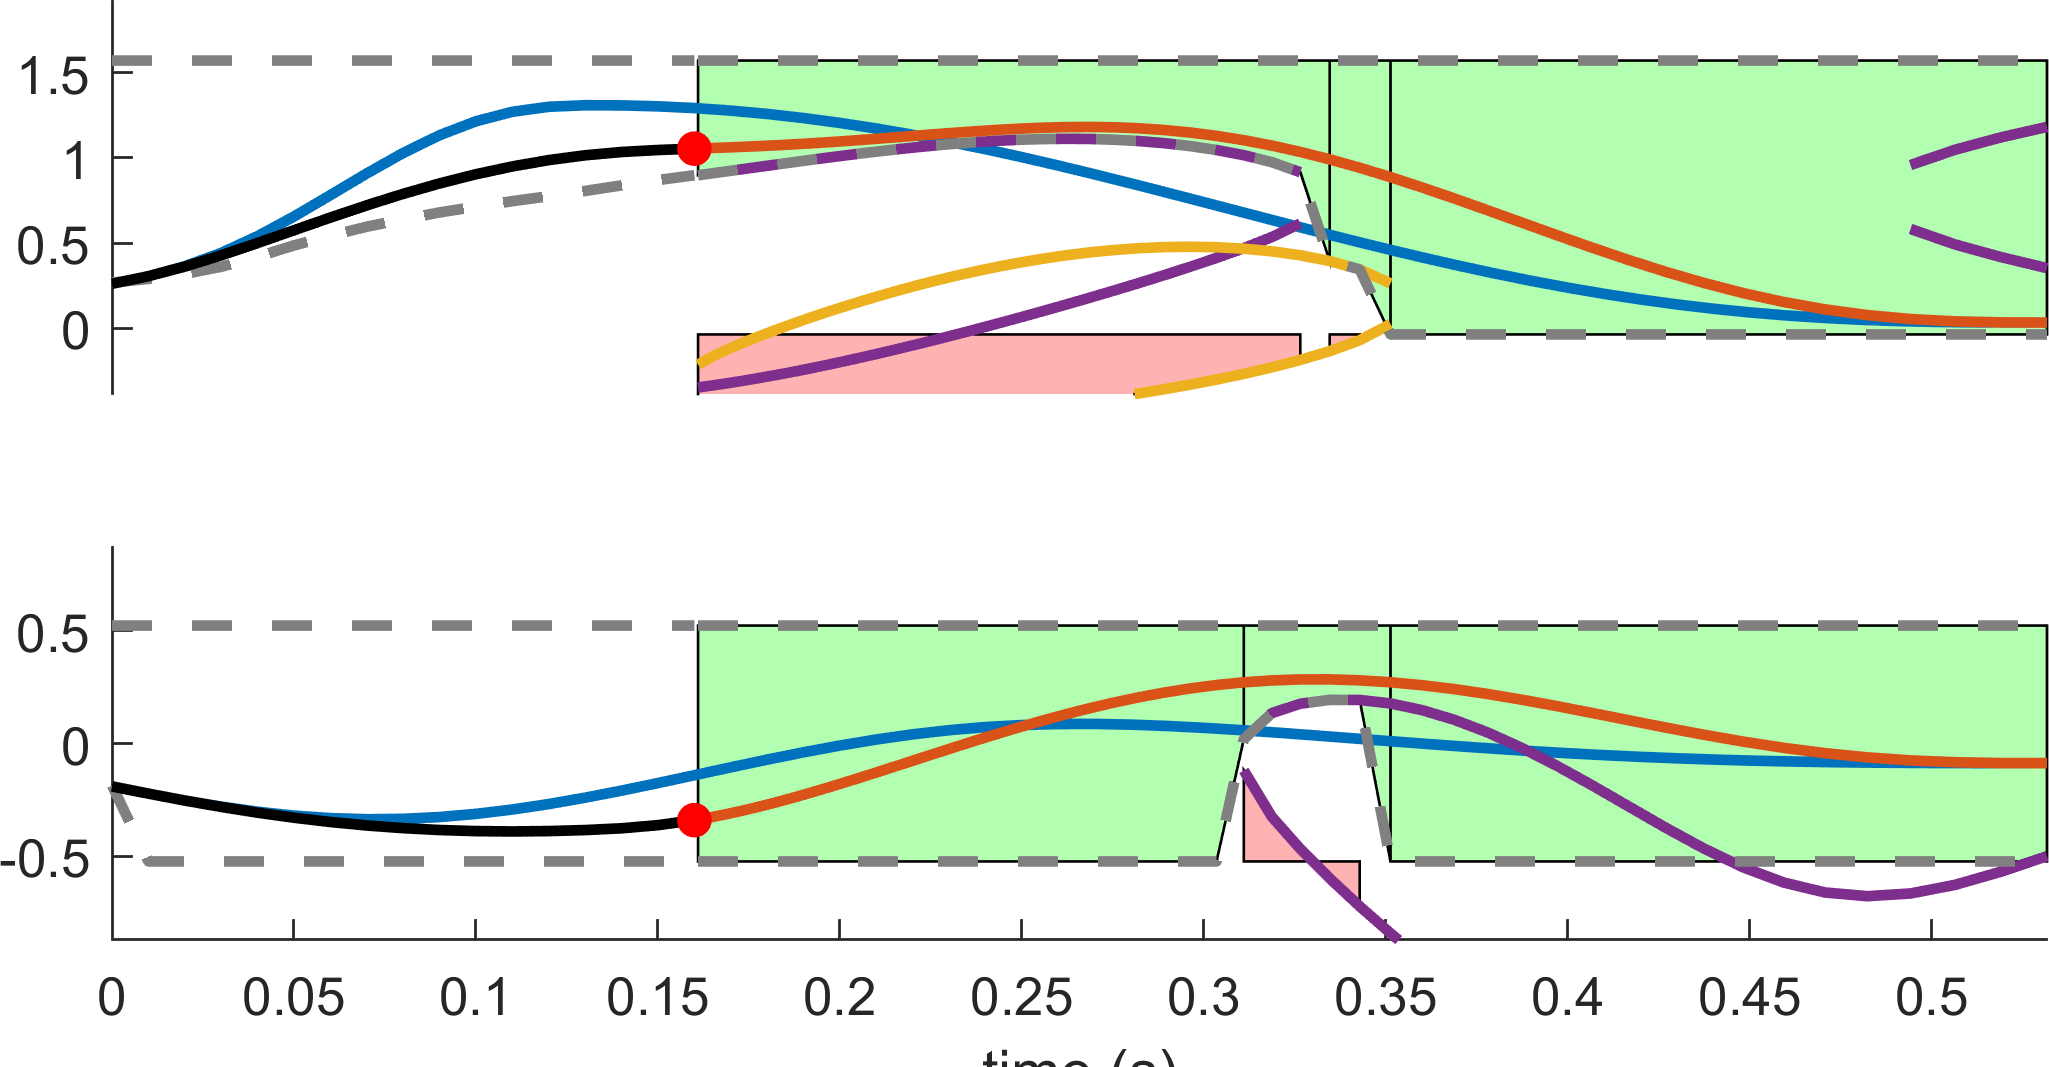
\includegraphics[width=\textwidth]{planning}
    \caption{Planning Algorithm Steps: Panels B and D
    show the generated knee and ankle trajectories respectively.  The planned
    trajectory (red) lies within the computed bounds (dashed gray).  In
    contrast, standard minimum jerk trajectories (blue) do not respect the
    bounds, thereby increasing the tripping hazard. Panels C and E show examples
    of inverse kinematics (IK) solutions for toe (purple) and heel (yellow)
    contact for the knee and ankle joints respectively. We use the IK solutions
    to generate bounded regions that the planned trajectory can safely traverse.
    We consider ground contact constraints for only the first half of the
    remaining swing duration after which we only consider joint angle
    constraints. We use Dijkstra's algorithm to select regions (green) that
    allow a path from the start point to the desired final point. Bounded
    regions that do not lie on the path are shown in red. Panel A shows the
    corresponding prosthesis motion.}\label{fig:planning}
\end{pagefigure}

To obtain reactive control of the prosthesis swing leg motion, we plan future
swing trajectories with a fast quadratic program (QP) operating at
\unit[100]{Hz}. The QP includes equality constraints, which ensure the
trajectories progress smoothly from the current position to the desired end
position, and inequality constraints, which avoid premature ground contact of
toe and heel of the prosthesis. Because in our formulation the QP can only solve
for one joint at a time, we first solve for the ankle trajectory assuming the
knee trajectory found in the previous time step, and then use this updated ankle
trajectory to solve for the new knee trajectory.

\Cref{fig:planning} provides more details of the actions of the trajectory
planner algorithm. For example, at a time of about \unit[150]{ms} into the swing
phase, the algorithm solves
\begin{align}
    \theta_\tn{k}^\textrm{toe bnd} 
        &= \left\{\theta_\tn{k} : \left\{p_\tn{OT}
            (\theta_\tn{h}, z_\tn{h}, \theta_\tn{k}, \theta_\tn{a})
            \right\}_\textrm{row 3} = 0 \right\} \\
    \theta_k^\textrm{heel bnd} 
        &= \left\{\theta_\tn{k} : \left\{p_\tn{OL}
            (\theta_\tn{h}, z_\tn{h}, \theta_\tn{k}, \theta_\tn{a})
            \right\}_\textrm{row 3} = 0 \right\}
\end{align}
at a set of sample times spanning the remaining swing trajectory to obtain a
planned knee trajectory (red trace in \cref{fig:planning}B).
Figures~\cref{fig:planning}C and E show the predicted inverse kinematics (IK)
solutions at characteristic points into the swing for the knee and ankle
respectively, with solutions leading to toe contact shown in purple and
solutions leading to heel contact shown in yellow. For each contact point, there
are typically two solutions, one lower bound, for which the joint angle cannot
cross from above, and one upper bound, for which the joint angle cannot cross
from below. 

Often, the valid leg configurations span disjointed regions in the configuration
space (green and red regions in \cref{fig:planning}B and D). Therefore, the
planner next identifies a valid sequence of regions for the trajectory to
traverse in a four step procedure.  First, the planner identifies critical
points along the predicted trajectory at which any bound activates or
deactivates. Second, at each critical point, the planner sorts the bound angles
from largest to smallest and iterates through them to define regions between
successive upper and lower bounds. Third, the planner defines a graph over the
regions with edge weights equal to the average squared angle minus the volume of
the child region. This cost favors a sequence of regions that are large and thus
safe to travel trough and avoids regions that require excessive joint flexion or
extension. Dijkstra's algorithm is then used to find a valid sequence of regions
that minimizes this cost~\citep{dijkstra1959note}. Finally, so that the
generated trajectories do not get too close to the identified bounds, a buffer
is added to the bounds. This buffer takes the form
\begin{align}
    \theta_\tn{buf} = \theta_\tn{buf}^0 \sin 
        \left(\pi \frac{t - t_0}{t_f - t_0} \right),
\end{align}
where $\theta_\tn{buf}^0$ is either \unit[5]{$^\circ$} or \unit[-5]{$^\circ$}
for lower and upper bounds respectively, $t$ is the future swing time, and $t_0$
and $t_f$ are the current and final swing times.

After identifying the bounded regions, the planner generates the trajectory for
a specific joint by solving a quadratic program. The trajectory of each joint is
represented by three, fifth-order polynomial splines,
\begin{align}
    \theta_1(t) &= a_{01} + a_{11} t + \cdots + a_{51} t^5 
        = [1 \ t \cdots t^5] a_1 \\ 
        T_0 &\le t < T_1 \\
    &\vdots \notag \\
    \theta_3(t) &= a_{03} + a_{13} t + \cdots + a_{53} t^5 
        = [1 \ t \cdots t^5] a_3 \\ 
     T_2 &\le t < T_F,
\end{align}
and solved for by the following QP,
\begin{align}
    a^* = \argmin_a \ \frac{1}{2} a^T (H_\theta + w H_{\dddot{\theta}}) a
    \label{eq:quadprog},
\end{align}
where $a = [a_1^T \ a_2^T \ a_3^T]^T$, $H_\theta$ and $H_{\dddot{\theta}}$
encode quadratic costs on angle and jerk respectively, and $w$ is a weight
parameter. The solution is subject to the inequality constraints
\begin{align}
    \theta(t) &\le \theta_\tn{max}(t), \ \forall t\\
    \theta(t) &\ge \theta_\tn{min}(t), \ \forall t\\
    \dot{\theta}(t) &\le \dot{\theta}_\tn{max}, \ \forall t\\
    \dot{\theta}(t) &\ge \dot{\theta}_\tn{min}, \ \forall t,
\end{align}
which ensure the trajectory lies within the identified bounds and respects
velocity limits, and to the equality constraints
\begin{align}
\theta(T_0) &= \theta_0 \\
\dot{\theta}(T_0) &= \dot{\theta}_0 \\
\ddot{\theta}(T_0) &= \ddot{\theta}_0 \\
\theta(T_F) &= \theta_F \\
\dot{\theta}(T_F) &= 0 \\
\ddot{\theta}(T_F) &= 0 \\
\theta_1(T_1) &= \theta_2(T_1) \\
\dot{\theta}_1(T_1) &= \dot{\theta}_2(T_1) \\
\ddot{\theta}_1(T_1) &= \ddot{\theta}_2(T_1) 
\label{eq:quadprog_last_constraint} \\
&\vdots \notag
\end{align}
which ensure the trajectory starts at the current and terminates at the desired
positions, velocities, and accelerations and that the splines join together
smoothly.  If the QP fails to find a trajectory that can satisfy the
constraints, the last found valid trajectory is reused for the next time step.
In addition, at the first iteration, the ankle trajectory planner uses the
output of the minimum jerk trajectory planner to solve the inverse kinematics
for the bounds. 

\subsection{Experimental Procedure}
We tested the ability of the proposed trip avoidance control to reduce the
incidence and severity of trips while walking with the powered transfemoral
prosthesis shown in \cref{fig:kinematics} To evaluate the performance of the
system, an able-bodied user walked with the prosthesis while attempting to
elicit trips by lowering the hip in swing. During the stance phase, the
prosthesis randomly decided to either use the proposed swing control or to use
standard minimum jerk trajectories that do not consider the tripping hazard. The
user was not aware of which controller would be used in the upcoming swing.  The
user completed a total of ten one minute walking trials.

We examined several outcomes for evaluating the control performance. First, we
examined the distribution of knee angles at the beginning of stance. Large knee
angles at the beginning of stance indicate premature landing due to toe-strike
instead of heel strike. Ideally, the landing angle is close to the desired final
angle of \unit[2]{degrees}. Second, we checked the integral of the ground
reaction force during swing. If this quantity is large, it indicates scuffing of
the toe on the ground. Finally, we examined the relationship between the hip and
toe heights during swing. If our controller is working as intended, the toe
height during swing should have a decreased sensitivity to the hip height.

\section{Results}
\begin{figure}[h]
    \centering 
    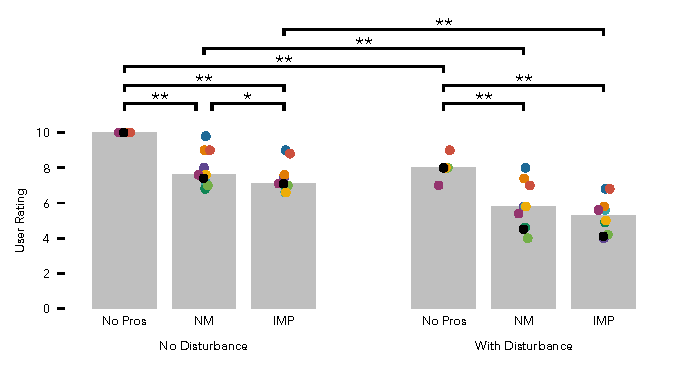
\includegraphics[width=\textwidth]{treadmill_vib_user_scores}
    \caption{Average user ratings across all trials in both the undisturbed and
    disturbed walking conditions when walking without the prosthesis (No Pros)
    and with the Neuromuscular (NM) prosthesis control and impedance (IMP)
    prosthesis control. Grey bars show the mean across subjects.  Statistical
    significance assessed by paired $t$-tests. $*$:~$p < 0.05$, $**$:~$p <
    0.01$, $***$:~$p < 0.001$.}\label{fig:treadmill_user_ratings}
\end{figure}
First, \cref{fig:treadmill_user_ratings} shows the user ratings of the different
conditions. We mandated that users rate the No Prosthesis/No Disturbance case
10/10 so that other conditions could be rated relative to this case. We see that
in both the no disturbance and disturbance cases, neuromuscular control was
rated significantly more preferably than impedance control. Neither control
could match the ratings given to the no prosthesis case. Introduction of the
disturbance caused a significant drop in user rating for all controllers. 

\begin{figure}[t]
    \centering 
    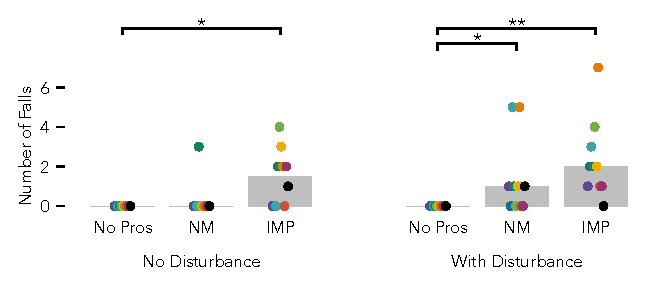
\includegraphics[width=\textwidth]{treadmill_vib_num_falls}
    \caption{Total number of falls across all trials in both the undisturbed and
    disturbed walking conditions when walking without the prosthesis (No Pros)
    and with the Neuromuscular (NM) prosthesis control and impedance (IMP)
    prosthesis control. Grey bars show the median number of falls across all
    subjects. Statistical significance assessed by Wilcoxon signed-rank test.
    $*$:~$p < 0.05$, $**$:~$p < 0.01$.}\label{fig:treadmill_exp_falls}
\end{figure}
Next, \cref{fig:treadmill_exp_falls} shows the number of falls in each
condition. Here we see that there was significant differences in the median
number of falls between impedance control and no prosthesis walking in the no
disturbance case and both impedance and neuromuscular walking in the disturbance
case. No significant differences were found directly between the neuromuscular
and impedance controllers.

\begin{figure}[b]
    \centering 
    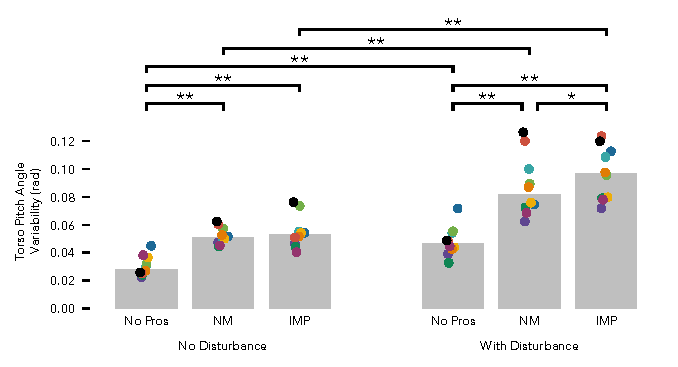
\includegraphics[width=\textwidth]{treadmill_vib_torso_var_x}
    \caption{Torso pitch angle variation. Angle variation calculated as the
    interquartile range of torso angles after the median torso angle trajectory
    over the strides in a trial is subtracted out. For the prosthesis trials, we
    report the average variation across the five trials for each condition.
    Grey bars show the mean across subjects.  Statistical significance assessed
    by paired $t$-tests. $*$:~$p < 0.05$, $***$:~$p <
    0.001$.}\label{fig:treadmill_exp_torso_var_x}
\end{figure}

\begin{figure}[t]
    \centering 
    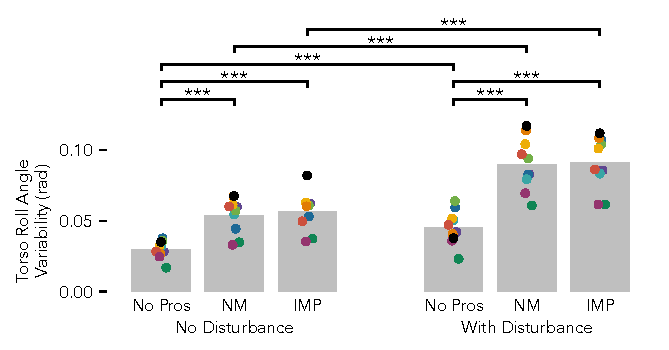
\includegraphics[width=\textwidth]{treadmill_vib_torso_var_y}
    \caption{Torso roll angle variation. Angle variation calculated as the inter
    quartile range of torso angles after the median torso angle trajectory over
    the strides in a trial is subtracted out. For the prosthesis trials, we
    report the average variation across the five trials for each condition.
    Grey bars show the mean across subjects.  Statistical significance assessed
    by paired $t$-tests.$***$:~$p < 0.001$.}\label{fig:treadmill_exp_torso_var_y}
\end{figure}

\Cref{fig:treadmill_exp_torso_var_x,fig:treadmill_exp_torso_var_y} show the
torso pitch and roll angle variability respectively. We see significant
differences between the no prosthesis and with prosthesis cases as well as the
no disturbance and with disturbance cases. There is also a significant increase
in torso pitch variability with the impedance control compared to the
neuromuscular control in the disturbance case.

\begin{table}[t]
  \begin{center}
    \begin{tabular}{lcc}
      Fall Types & Neuromuscular & Impedance \\
      \midrule
      Fall Forward &  1 &  0 \\
      Fall Backwards &  6 &  4 \\
      Fall Left &  1 &  0 \\
      Fall Right &  0 &  3 \\
      Missed Stance / Swing Transition &  3 &  0 \\
      Missed Stance 2 / Stance 3 Transition &  0 &  7 \\
      Knee Collapse & 0 & 15 \\
      Swing Trip & 4 & 12 \\
    \end{tabular}
  \end{center}
  \caption{Tally of observed reasons for falls across all subjects and across
  both the undisturbed and disturbed walking conditions. Falls were manually
  classified based on video and logged prosthesis data. An individual fall can
  be assigned more than one reason.}\label{tab:treadmill_exp_fall_reasons}
\end{table}
Finally, \cref{tab:treadmill_exp_fall_reasons} shows a tally of the reasons for
the observed falls with each controller type when using preferred parameters.
We manually determined the reason for each fall by analyzing video recordings,
motion capture data, and logged prosthesis data. The first four categories refer
to general losses of balance resulting in a fall in the four cardinal
directions. Backward falls generally resulted from the treadmill suddenly
stopping when the prosthesis stance leg was still in front of the body, causing
a loss of balance backwards. The falls forward, left and right were generally
more ambiguous in their cause, but may be due to improper leg placement. 

The missed stance/swing transitions in the neuromuscular control were caused
when subjects did not allow the leg angle to cross the $90^\circ$ threshold set
in stance/swing state machine (compare \cref{fig:stance_swing_state_machine}).
The missed stance 2/stance 3 transitions occurred with impedance control if the
user did not dorsiflex the ankle sufficiently to trigger the transition. This
could cause the knee to produce an extension torque in late stance, making it
difficult to enter the swing phase (compare \cref{fig:treadmill_imp_fit}). As
shown in \cref{fig:treadmill_exp_phase_success}, the rate at which the impedance
conrtroller failed to transition through all three stance phases significantly
increased with the introduction of disturbances.
\begin{marginfigure}[-2.5in]
    \centering 
    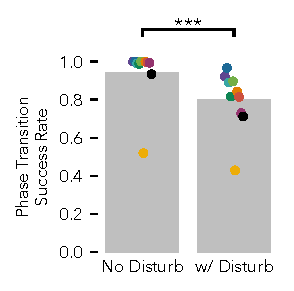
\includegraphics[width=\textwidth]{phase_success}
    \caption{Fraction of steps for which impedance control successfully
    transitions through all three stance phases. Disturbances significantly
    decrease the transition success rate. Grey bars show the mean success rate
    across all users. Statistical significance assessed by paired $t$-test.
    $***$:~$p < 0.001$.}\label{fig:treadmill_exp_phase_success}
\end{marginfigure}

In contrast, the knee collapse fall type was triggered in impedance control if
the user dorsiflexed the ankle too early causing a premature switch to the third
phase of stance. In this phase, knee torque typically trends towards zero to
allow for passive flexion of the knee heading into swing. However, in the case
of a premature switch to the push-off phase, these near-zero knee torques can
cause the knee to suddenly collapse under the user's weight. 

The last cause of falls, trips during swing, occurred when using both
controllers, but 3x more often with impedance control than with neuromuscular
control. Many of the swing trips for impedance control were also preceded by a
missed stance 2/stance 3 transition. Others occurred when kinematics were
drastically changed by the disturbance. For example, several swing trips
occurred after a sudden acceleration of the treadmill caused the stance step
length to dramatically increase, thereby altering kinematics at toeoff and in
swing, and leading to the toe hitting the ground mid-swing.

\begin{figure}[b]
    \centering 
    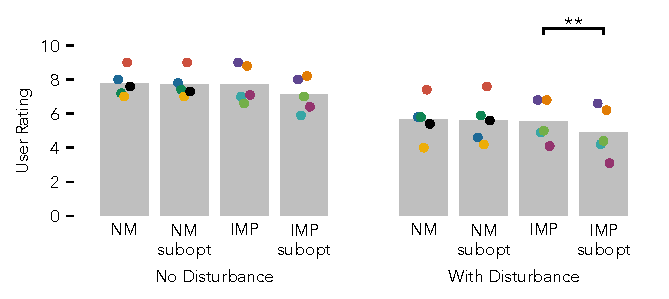
\includegraphics[width=\textwidth]{treadmill_vib_user_scores_subopt}
    \caption{Comparison of user scores of optimal versus suboptimal parameters
    for the neuromuscular and impedance control strategies. Grey bars show the
    mean user rating across subjects. Statistical significance assessed by
    paired $t$-tests. $**$:~$p <
    0.01$.}\label{fig:treadmill_exp_user_ratings_subopt}
\end{figure}
Finally, we look at the effect of using suboptimal controllers on user ratings
and falls. \Cref{fig:treadmill_exp_num_falls_subopt} shows the median ratings of
each the preferred and suboptimal parameters for each controller. For
neuromuscular control, we see no significant difference between the preferred
controller from day 4 and the suboptimal controllers. In fact for the
neuromuscular control with disturbances, 4 out of 5 users slightly preferred the
suboptimal control from day 5. On the whole, choosing a suboptimal set of
parameters seemed to have a larger effect on impedance control with 4 out of 5
subjects preferring the optimal to suboptimal parameters with out disturbances
and all five subjects preferring the optimal impedance parameters to the
suboptimal parameters in disturbed case.

\Cref{fig:treadmill_exp_num_falls_subopt} shows the median number of falls
garnered by optimal and suboptimal parameters. In the disturbance case we see a
increase in the median number of falls with the suboptimal parameter sets over
the preferred parameter sets. However this difference was not significant.

\begin{figure}[t]
    \centering 
    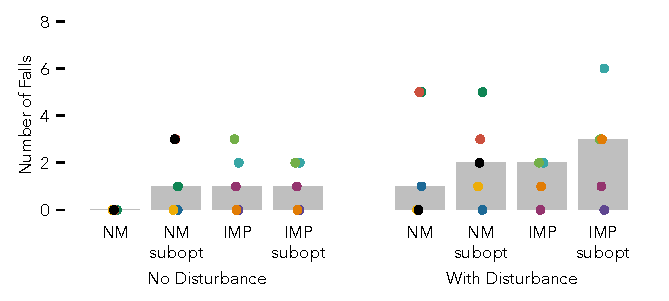
\includegraphics[width=\textwidth]{treadmill_vib_num_falls_subopt}
    \caption{Comparison of number of falls of optimal versus suboptimal
    parameters for the neuromuscular and impedance control strategies. Grey bars
    show the median number of falls across subjects. Statistical significance
    assessed by Wilcoxon signed-rank
    test.}\label{fig:treadmill_exp_num_falls_subopt}
\end{figure}

\section{Discussion}

We presented initial work toward a real-time reactive control of powered
prostheses to help amputees avoid tripping in the swing phase of gait. At any
time during swing, the proposed control uses a laser range finder and an
inertial measurement unit to estimate the current pose of the prosthesis,
predicts the future hip angle and height based on trained Gaussian process
models, and then plans new knee and ankle joint trajectories that ensure neither
the toe nor heel contacts the ground prematurely. Our results indicate the
proposed control approach can substantially reduce the incidence of trips and
reduce the severity and frequency of toe scuffing.

To the best of our knowledge, this work is the first demonstration of lower limb
prosthetic control that integrates perception feedback in real-time and that
proactively ameliorates the falling hazard amputees face. Previous research in
this area has largely focused on detecting stumbles \emph{after} they have
occurred. For example, \citet{lawson2010stumble} and \citet{shirota2014recovery}
have proposed classifiers that can detect trips during swing and predict whether
a lower or raising strategy should be used in response. Similarly,
\citet{zhang2011towards} have proposed a method that can detect stumbles and
classify them as trips during swing or slips during stance. However, these
previous studies have not proposed concrete control actions to preempt stumbles
or to properly react in the event that a stumble is detected. Our results
motivate further research into such proactive and reactive approaches, closing
the perception-action loop for improving gait robustness with robotic
prostheses.

Several avenues for future work exist. First, in our current study only one
able-bodied user tested the proposed control. Further experiments with amputee
subjects are needed to verify the system provides benefits to this population.
For instance, amputees accustomed to walking with passive prostheses show
significantly altered hip kinematics~\citep{jaegers1995prosthetic}, which could
affect the control behavior. However, the proposed control should be able to
properly adapt to these behavior differences, as the Gaussian process models are
trained for specific users. Second, although trips during swing are one of the
most common failure modes we encounter with our powered prostheses, these events
are still rare and many hours of normal walking are required to observe a
sufficient number of trips and compare controllers. As a result, we actively
induced trips by sudden drops in hip height during swing, which does not exactly
reflect the situations in which trips occur.  Specifically, trips can happen due
to subtle changes in leg kinematics, and it remains to be seen in experiments if
our approach can avoid trips in these more subtle situations.

At the implementation level, there is also room for further exploration. To keep
the  computational costs low, we used quadratic programs that iterate between
finding solutions for the ankle and knee joints. While this iterative approach
is fast when compared to trajectory optimization methods that deal with multiple
joints simultaneously, the iterations occasionally get stuck when the planner
for one joint trajectory cannot find a solution based on the assumed fixed
trajectory of the other joint. Moreover, if a solution cannot be found, the
current approach simply reuses the last identified trajectory, rather than
moving the trajectory to be more safe, even if it cannot fully satisfy the
bounds. It seems worthwhile to investigate whether non-convex trajectory
optimization methods such as CHOMP \citep{ratliff2009chomp}, in which the bounds
are represented as soft rather than hard constraints, can help solve for the
knee and ankle trajectories simultaneously without sacrificing computational
speed.

In addition, several technical simplifications can be considered to bring this
technology closer to commercialization. We used an accurate and expensive laser
distance sensor, eyeing future research in obstacle scanning and avoidance
capabilities. However, for simple ground plane avoidance, inexpensive infrared
distance sensors such as those used by \citet{scandaroli2009estimation} are
likely sufficient. It may also be possible to simplify the trajectory planning
phase by, for example, forgoing formal guarantees on satisfying bounds and
instead relying on heuristics to increase knee and ankle flexion and adjust
timing in response to decreased hip height during swing.

Our immediate goal, however, is to generalize the presented approach to
incorporating perception in control beyond the avoidance of flat ground. We are
currently investigating the approach's ability to plan trajectories around
obstacles that are scanned by the laser range finder. Previous studies such as
\citet{mohagheghi2004effects} with able-bodied subjects have shown that vision
plays a crucial role in both planning and control of the lower limb motion over
obstacles. We also envision using the approach to target objects instead of
avoiding them. For example, a prosthetic leg could scan, recognize, and target
secure foot holds and stair treads, or provide enhanced sports capabilities by
targeting and kicking a ball.

